\chapter{Estrutura e funcionamento do Framework\label{cap:detalhamento-projeto}}

    \section{Processo de instalação\label{sec:processo-instalacao}}
        O \emph{Framework Lothus\{PHP\}} permite ao desenvolvedor a possibilidade de escolha entre dois níves de aplicação. O primeiro nível permite a instalação do \emph{Framework} da forma mais simples, instalando utilitário focados em um desenvolvimento direcionado ao backend do projeto, integrando facilidade a troca de informações com o banco de dados, desenvolvimento através do MVC, URLs amigáves e sistemas de templates.

        Essa instalação é feita através do repositório remoto \emph{Github}, que se encontra no seguinte endereço online:

        \emph{https://github.com/guilouro/Lothus-PHP}

        O Github permite duas formas de download de um projeto: fazendo o downloand de um arquivo comprimido em .zip diretamente do site ou utilizando um sistema de versionamento de arquivos para fazer o clone do mesmo. Neste projetos iremos usar o \emph{Git} como sistema de versionamento. Para fazer o clone utilizando o git executamos a seguinte linha de comando no terminal Unix ou cmd Windows:

        \textbf{\$ git clone https://github.com/guilouro/Lothus-PHP.git}

        Ao executar essa linha de comando, uma nova pasta será criada com o nome de Lothus-PHP. Dentro desta nova pasta estará todo o projeto para iniciar o desenvolvimento utilizando o \emph{Framework Lothus\{PHP\}}. O próximo capítulo será responsável pela apresentação das pastas existentes dentro do projeto.




    \section{Estrutura de pastas\label{sec:estrutura-pastas}}
        Neste capítulo será apresentado a estrutura de pastas do \emph{Framework Lothus\{PHP\}} juntamente com o detalhamento de cada funcionalidade do projeto.

        \begin{figure}[!htb]
            \centering
            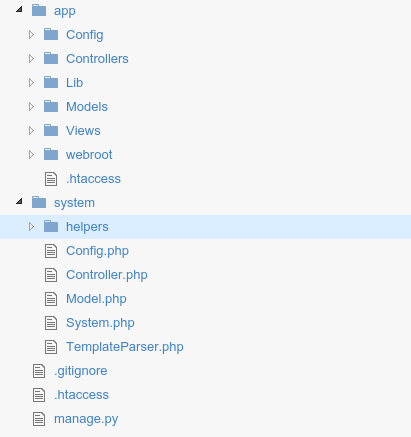
\includegraphics[scale=0.8]{pastas.jpg}
            \caption{\small Estrutura do projeto}
            \label{cap:sass}
        \end{figure}

    \section{Divisão Backend - frontend\label{sec:back-front}}

        \subsection{Comandos do Grunt\label{sub:comandos-grunt}}

    \section{System\label{sec:estrutura-pastas}}

    \section{Model\label{sec:estrutura-pastas}}

    \section{View\label{sec:estrutura-pastas}}

    \section{View\label{sec:estrutura-pastas}}

    \section{Template\label{sec:estrutura-pastas}}
